%%%%%%%%%%%%%%%%%%%%%
%								%
%	APENDICES					%
%								%
%%%%%%%%%%%%%%%%%%%%%

\appendix
\newpage
\chapter{Apendice A}
\label{Apendice A}
Acá van los apéndices, aprovechando...

Nota: los archivos memoria.algo (con "algo" distinto de "tex") se generan automáticamente al compilar, algunos errores con la bibliografía pueden solucionarse borrándolos y re-compilando.

\chapter{Teoria de Grafos}\label{ap:apendice_B}
inicio de mi grafo \cite{book_introduction_graph_theory}
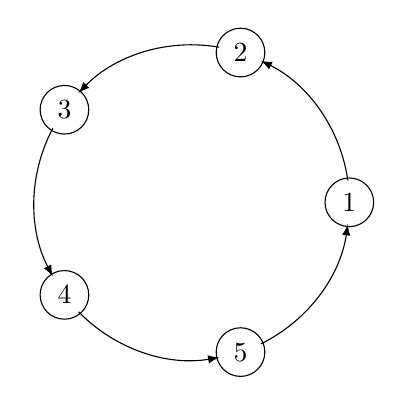
\begin{tikzpicture}

\def \n {5}
\def \radius {2cm}
\def \margin {8} % margin in angles, depends on the radius

\foreach \s in {1,...,\n}
{
test
  \node[draw, circle] at ({360/\n * (\s - 1)}:\radius) {$\s$};
  \draw[->, >=latex] ({360/\n * (\s - 1)+\margin}:\radius) 
    arc ({360/\n * (\s - 1)+\margin}:{360/\n * (\s)-\margin}:\radius);
}
\end{tikzpicture}

Final de mi grafo

\chapter{Catalog management handled with relational databases}\label{ap:apendice_C}

\begin{figure}[h!]
	\centering
	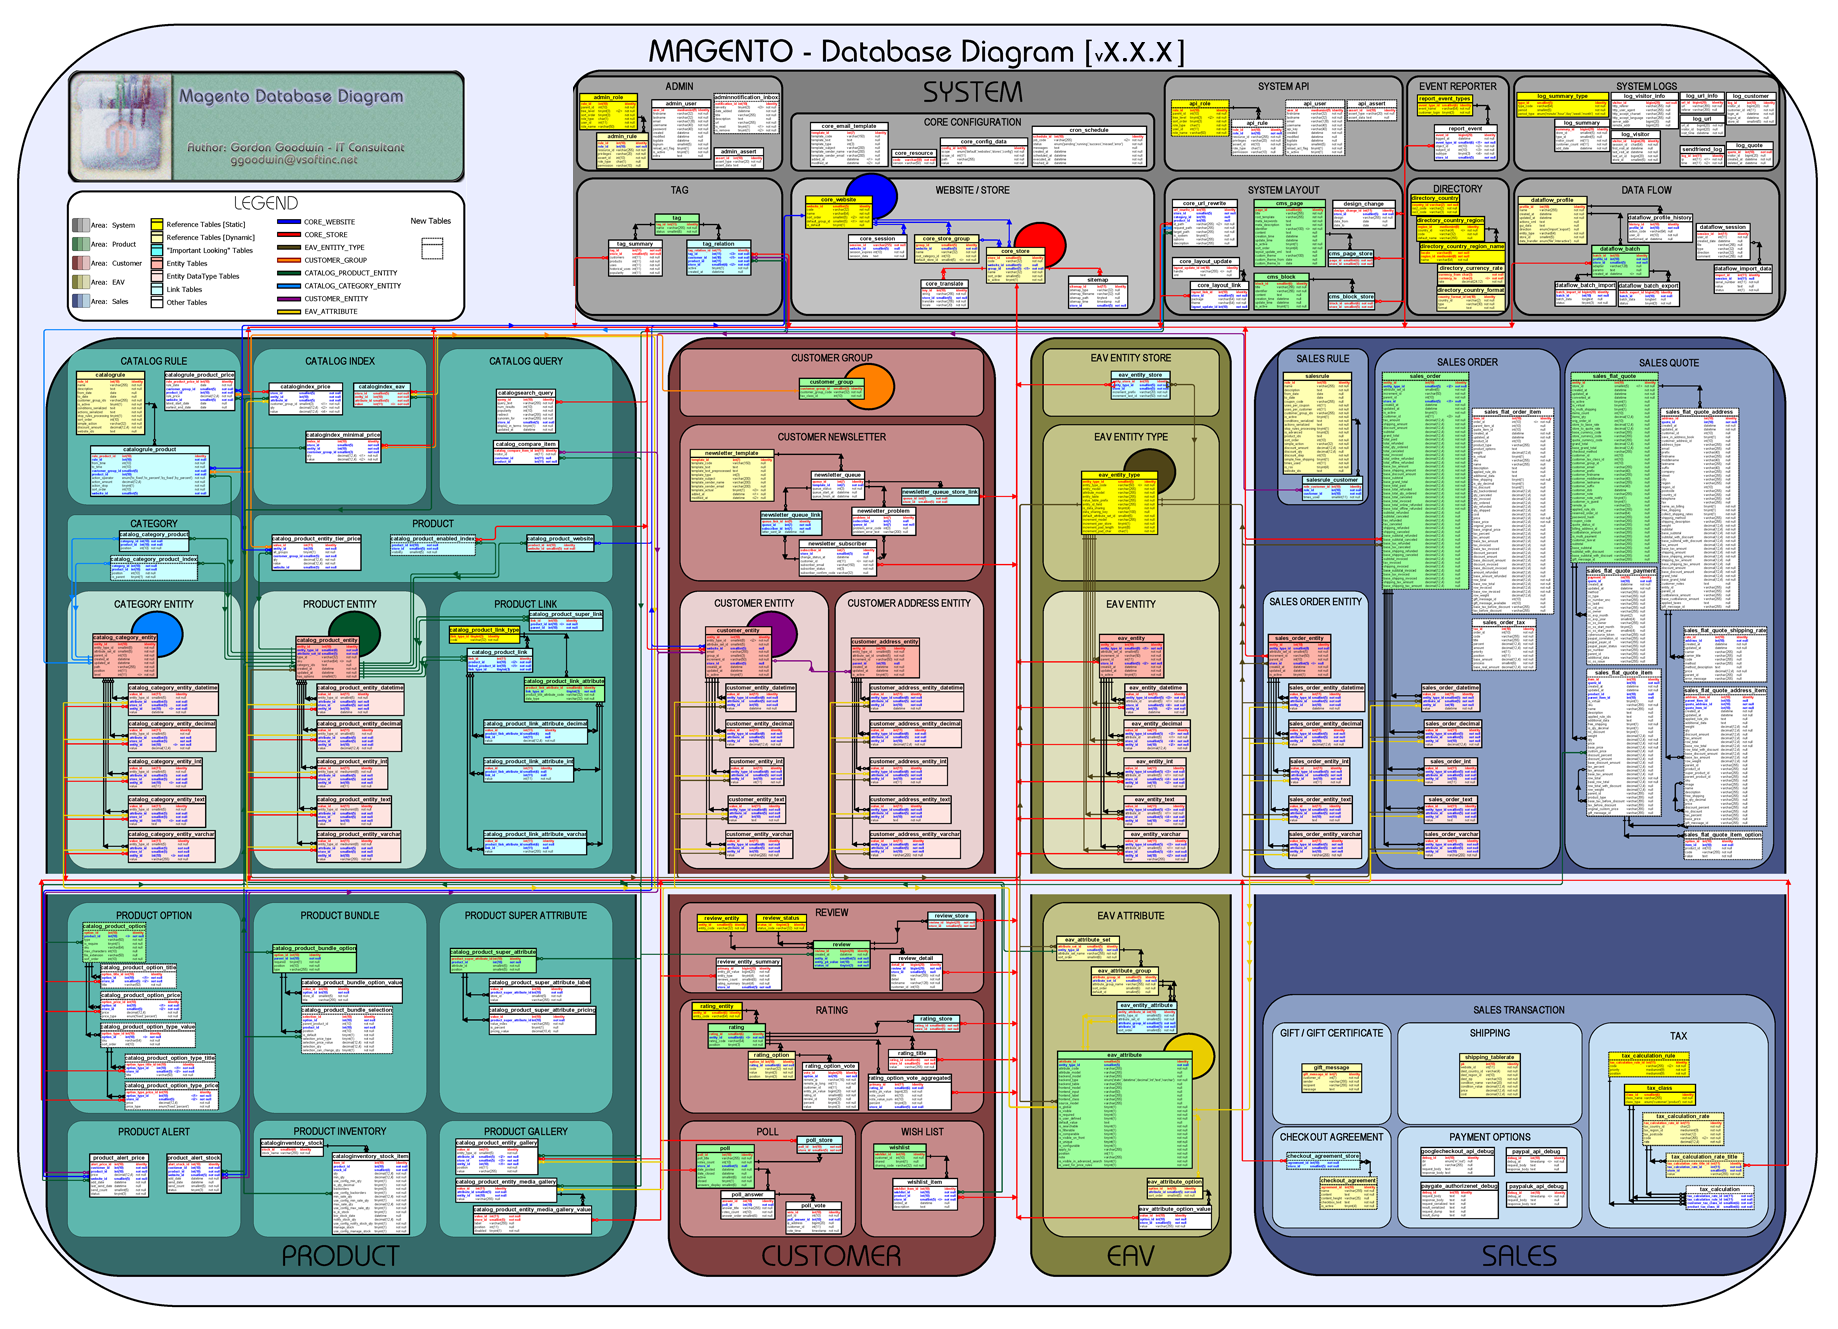
\includegraphics[width=0.8\textwidth]{figuras/apendice/magento_sample_database_diagram.png}
	\caption{schemas of Magento e-commerce framework.}
	\label{ap:figure:catalog_magento}
\end{figure}

\begin{figure}[h!]
	\centering
	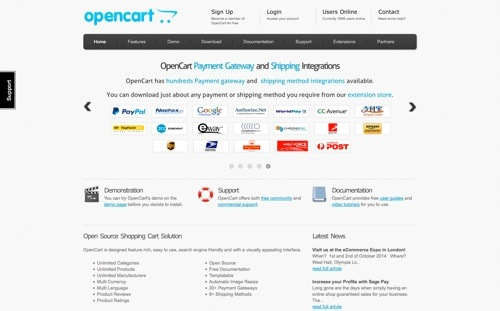
\includegraphics[width=0.5\textwidth]{figuras/apendice/openCartWebsite.jpg}
	\caption{schemas of the Apache's OfBiz.}
	\label{ap:figure:catalog_ofbiz}
\end{figure}